\chapter{Background}\label{chapter:background}
\section{Virtualization}
Virtualization is a technology that allows the creation of isolated virtual environments also known as 
Virtual Machines that run on the same physical server \cite{virtualization_review}. Each VM has its own 
operating system and acts as an independent physical computer. The VMs are called "guests" and the 
physical server is called "host". Virtualization is crucial for the \ac{IaaS} model offered by 
cloud providers, as it provides various advantages \cite{virtualization_review}. It improves resource and 
cost efficiency by dividing the physical server into multiple isolated instances, each tailored to 
different workload needs. This reduces the amount of unused capacity that occurs when a server is dedicated 
to just one task. \\
The main component that handles the necessary tasks for virtualization is the \ac{VMM} 
also called hypervisor \cite{nitro_whitepaper}. Most of the instructions that are executed by the virtual 
machines run natively on the CPU and do not require intervention from the \acs{VMM}, such as arithmetic 
operations. 
However, there is a class of privileged instructions that guests can not directly execute on the CPU, 
such as I/O operations. When such an instruction is encountered, the CPU raises a 
trap, which signals to the \acs{VMM} to intervene and emulate the behavior of the instruction \cite{nitro_whitepaper}.  
After the emulation is finished, the control is then given back to the guest OS, 
which is unaware of the underlying emulation. Several optimization techniques have been introduced 
to reduce virtualization overhead, which will be briefly outlined. \\
Virtualization cannot be carried out by the VMM alone, as it does not virtualize hardware and therefore 
can not grant the guests access to the underlying hardware devices such as network interfaces, storage drives, 
and input peripherals. Device models are required for this \cite{nitro_whitepaper}. They are basically 
software components that communicate with the shared hardware and expose multiple virtual device 
interfaces to the VMs. Device models, along with other management software, run in a special 
privileged virtual machine called management domain, which represents the host's operating system and 
has access to all the underlying hardware. This domain is called domain zero or dom0 in the Xen project,
and root/parent partition in the Hyper-V project \cite{nitro_whitepaper}. Since the device models are 
software-based, they compete for for CPU and other system resources along with the existing VMs and 
can negatively affect the performance of the guests. 
The following figure summarizes the architecture of a traditional virtualization system. 
\begin{figure}[H]
  \centering
  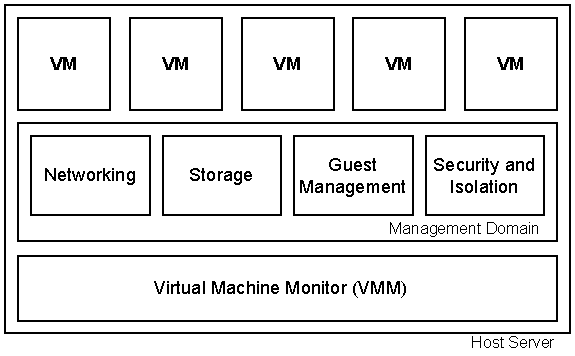
\includegraphics[width=10cm, height=6cm]{figures/traditional_hypervisor.pdf}
  \caption{Architecture of traditional virtualization Solution}
  \label{fig:hyper}
\end{figure}

\subsection{Evolution of Virtualization Solutions}
Virtualization technology has evolved significantly over the last decades. It started with full software virtualization, 
where the guest OS is unmodified and "unaware" of the virtual environment. Privileged instructions 
are trapped by the CPU, and the hypervisor emulates the sensitive instructions using 
binary translation \cite{virtualization_gregg}. This is, however, very slow and can make the host applications
run 2x to 10x slower \cite{virtualization_gregg}. \\
Then, paravirtualization was introduced, where the guest OS is modified to interact directly with the 
hypervisor via "hypercalls", removing the abstract emulation layer. The downside of this approach is that it introduces additional complexity, 
as it requires modifications to the guest operating system \cite{hvm}.\\ 
The next major leap was hardware-assisted virtualization (HVM), which introduced virtualization support 
directly on the hardware level by providing highly efficient and fast virtualization commands. 
This provides a significant improvement in comparison to the previous virtualization 
techniques, as it reduces the involvement of the host system in handling privilege and address translation
space tasks \cite{hvm}. Intel offers this under the Intel VT-x technology that provides virtualization of CPU and memory.
Another important example is Single Root Virtualization (SR-IOV) \cite{nitro_whitepaper}, which is a technology that allows physical 
PCI devices, such as Network Interface Card (NIC) to expose multiple virtual devices to the hypervisor. 
The hypervisor can then provide the different virtual machines with direct hardware access to these virtual 
devices, which significantly increases the I/O performance. 

\subsection{The AWS Nitro System}
The Nitro System is a result of a multi-year incremental process of AWS re-imagining the virtualization 
technology in order to optimize it specifically for their EC2 data centers \cite{nitro_whitepaper}. 
The main idea was to decompose the software components, i.e., the device models, 
that run on the management domain and offload them to independent purpose-built server components. 
This helps minimize the resource usage caused by software running in the management domain, effectively 
allowing a near "bare-metal" performance. Figure \ref{fig:nitro} depicts the new AWS
architecture for virtualization. 
\begin{figure}[H]
  \centering
  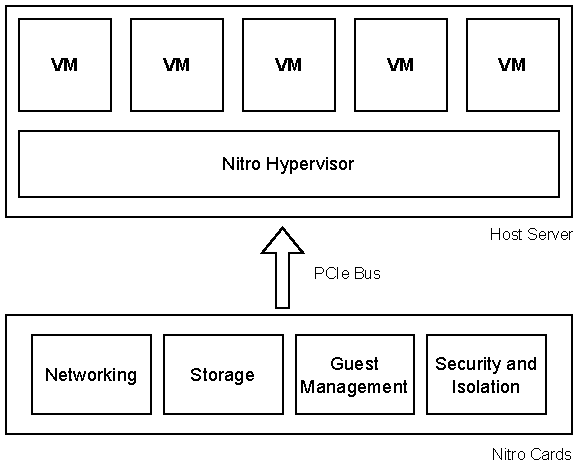
\includegraphics[width=10cm, height=7.5cm]{figures/nitro}
  \caption{Architecture of the AWS Nitro System \cite{nitro_whitepaper}}
  \label{fig:nitro}
\end{figure}
\noindent
There are three main components in the AWS Nitro System. 
\subsubsection{The Nitro Cards}
Nitro cards are dedicated hardware components that operate independently from the EC2's server main board 
(CPU and memory) and are physically attached to it via PCIe. They "implement all the outward-facing 
control interfaces used by the EC2 service" responsible for provisioning and managing compute, memory, 
and storage \cite{nitro_whitepaper}. They provide all I/O Interfaces as well, such 
as the ones for storage and networking. These cards employ the previously explained SR-IOV technology to 
provide direct hardware interfaces to the VMs. Examples of Nitro cards are Nitro cards for I/O and 
Nitro Controller, which provides the hardware root of trust of the Nitro System. 

\subsubsection{The Nitro Security Chip}
The Nitro Security Chip extends the hardware root of trust and control over the system's main board. It
is managed by the Nitro Controller and plays a crucial role in enabling 
AWS to offer bare-metal instances. Bare-metal instances provide direct access to the physical CPUs and memory 
of the physical server. They are useful mainly for licensing-restricted business-critical applications, or for 
specific workloads that require direct access to the underlying infrastructure. \\ 
In virtualized environments, the hypervisor is responsible for securing the host's hardware assets. 
However, in bare metal modes, when no hypervisor is present, the Nitro Security Chip 
assumes this role and ensures the security of the system firmware from tampering attempts through the system 
CPUs \cite{nitro_whitepaper}. 

\subsubsection{The Nitro Hypervisor}
The third component is the AWS Nitro Hypervisor, which has significantly fewer responsibilities than traditional
hypervisors, as most virtualization tasks are offloaded to the Nitro cards. It has three main functions.
It is responsible for partitioning memory and CPU by using the virtualization commands provided by the 
processor. It is also in charge of assigning the virtual hardware interfaces provided by 
the Nitro cards to the Virtual Machines and handling the machine management commands that come from 
the Nitro Controller (start, terminate, stop, etc.) \cite{nitro_whitepaper}. 

\section{Simultaneous Multi-threading}
Before we dive into \ac{SMT}, it is important to understand which problem it  
tries to solve and what the motivation behind it is. \\
A processor consists of a few hundred registers, load/store units, and a couple of multiple arithmetic units. 
The main goal is to keep all these resources as busy as possible. Multiple techniques have been 
employed to achieve this, such as instruction pipelining, superscalar architecture, and out-of-order execution 
\cite{SMT_Maximizing_on_chip_parallelism}.
Pipelining is a technique that breaks down the execution of an instruction into several distinct 
stages, with each stage using separate hardware resources \cite{SMT_under_the_hood}. During each CPU cycle, 
instructions advance from one stage to another. This allows the CPU to work on multiple instructions 
simultaneously, each being on a different stage. In a perfect scenario, where all instructions are 
independent, the processor can work simultaneously on \begin{math}n\end{math} instructions, 
with \begin{math}n\end{math} being the depth of the pipeline, i.e., the number of stages. 
The following table depicts a simple example of a five-stage pipeline. At the fifth clock cycle, 
the CPU is simultaneously working on five instructions.  

\begin{figure} [H]
\centering
\begin{tabular}{c|ccccccc}
\toprule
\diagbox[width=3.5cm]{Instr. No.}{Clock Cycle} 
  & \textbf{1} & \textbf{2} & \textbf{3} & \textbf{4} & \textbf{5} & \textbf{6} & \textbf{7} \\
\midrule
1 & IF  & ID  & EX  & MEM & WB  &     &     \\
2 &     & IF & ID  & EX  & MEM & WB  &     \\
3 &     &     & IF & ID  & EX  & MEM & WB  \\
4 &     &     &     & IF  & ID  & EX  & MEM \\
5 &     &     &     &    & IF  & ID  & EX  \\
\bottomrule
\end{tabular}
\caption{Basic five-stage pipeline (IF = Instruction fetch, ID = Instruction decode, EX = execute  MEM = memory read, WB = Write back to memory)}
\label{fig:table}
\end{figure}
\noindent
Modern processors are also superscalar. This means that each processor can start executing more 
than one instruction per cycle by dispatching them to different execution units \cite{SMT_Maximizing_on_chip_parallelism}. 
Issue width is an important characteristic of modern CPUs, and it represents 
the maximum number of instructions that can be started in a single clock cycle.
Although these optimizations significantly increase the processor throughput, the dependency  
between the instructions and the long latency operations of the executing threads limits the usage of the 
available execution resources \cite{SMT_Maximizing_on_chip_parallelism}. Out-Of-Order execution partially 
solves this problem, but it is still not enough, as it still dispatches instructions from the same thread, where 
the dependency between the instructions is inherently high. 
The wastages that occur on the processor can be categorized into two categories: Horizontal and 
vertical waste \cite{SMT_Maximizing_on_chip_parallelism}. 
Horizontal waste occurs when the CPU is not able to fully saturate the issue width of the processor. 
Vertical waste occurs when the processor is not able to start any instruction at all on a given cycle
because of the dependency to the executing instructions or delays such as memory latency. 
Traditional multithreading addresses this issue by switching to a different thread whenever 
the currently executing one stalls. This approach, however, only mitigates vertical waste, as 
it still issues instructions from only one thread at any given cycle \cite{SMT_Maximizing_on_chip_parallelism}.
\begin{figure}[H]
    \centering
    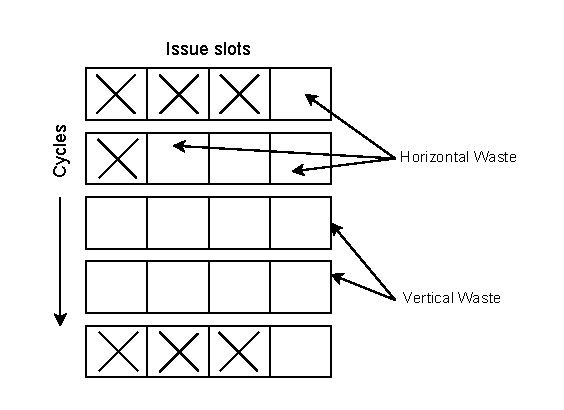
\includegraphics[width=10cm, height=7.5cm]{figures/cpu_wastages}
    \hspace{-2.5cm}
    \caption{Vertical waste vs. horizontal waste}
    \label{fig:cpu}
\end{figure}
\noindent
This is where \acl{SMT} comes into play. \acs{SMT} is a technique that helps enhance the overall efficiency of superscalar CPUs 
by improving the parallelization of computation \cite{SMT_under_the_hood}. This technology allows the 
physical core to dispatch instructions from more than one thread per cycle without requiring 
a context switch \cite{SMT_Maximizing_on_chip_parallelism}, effectively transforming each physical core into two (or more) "logical" cores. The idea is that instructions from different
threads provide greater independence, which results in a better utilization of the core's execution 
resources \cite{SMT_under_the_hood}.
To achieve this, some processor resources are duplicated, 
e.g., those that store the architectural state, such as registers and program 
counters \cite{SMT_under_the_hood}. However, the logical 
cores still share the same execution resources, which can create contention, especially if both threads have 
the same workload nature, e.g., both are float heavy \cite{SMT_modeling_resource_contention}. 
\begin{figure}[H]
    \centering
    \hspace*{-2cm} 
    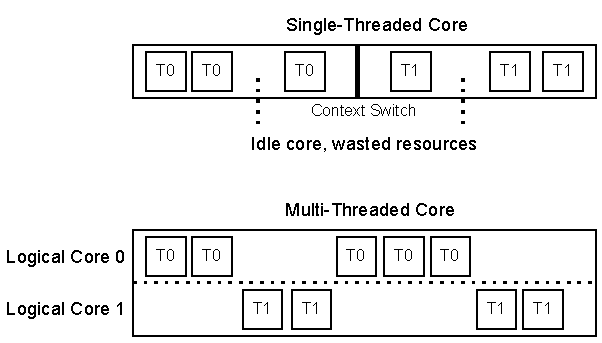
\includegraphics[width=10cm, height=6cm]{figures/single_vs_multithreaded}
    \caption{Single-Threaded Core vs. Multi-Threaded Core}
    \label{fig:all}
\end{figure}
\noindent
Both Intel and AMD implement this technology in their modern CPUs, providing two threads per physical core. 
Intel brands it as Hyper-Threading, while AMD uses the standard term \ac{SMT}. In the AWS dedicated hosts that run on an Intel or 
AMD CPU with hyperthreading enabled, the number of vCPUs is always equal to the double of the number of 
physical cores, with each vCPU corresponding to a hyperthread. This, however, opens up the possibility 
for CPU contention, if two virtual machines have access to vCPUs that share the same underlying physical core. 
Unlike Intel and AMD CPUs, AWS-designed Graviton processors, built around the ARM architecture, 
do not support hyper-threading and expose one execution context, i.e., vCPU for 
each physical core \cite{graviton}. This allows for a better isolation between the different tenants as 
there is no resource sharing between the different vCPUs apart from the last level cache and the memory 
system \cite{graviton}. 

\section{Dynamic Voltage and Frequency Scaling (DVFS)}
DVFS is a technique that allows the CPU to adjust its frequency based on the 
workload. When executing computationally intensive tasks, it allows the processor to jump to a 
higher frequency. Conversely, for light workloads or when the processor is idle, a lower clock rate 
is adopted. The goal is to create a balance between performance and energy efficiency. \\
Intel implements this technology under the name Intel® Turbo Boost Technology \cite{intelTurboBoost}. 
Its latest version allows frequency scaling on a per-core basis. Modern AMD processors also support 
similar per-core granularity through Precision Boost 2 \cite{amdPrecisionBoost2}. Frequency 
increases are, however, subject to certain conditions: The processor ensures that pre-defined temperature, 
as well as power consumption limits are not exceeded. In cloud environments, this behavior can potentially 
lead to performance degradation when the processor is forced to lower a core’s frequency from its peak 
level due to increasing power usage and processor temperature, caused by busy neighbors. 